\documentclass[conference]{IEEEtran}
\IEEEoverridecommandlockouts

\usepackage{cite}
\usepackage{amsmath,amssymb}
\usepackage{graphicx}
\usepackage{booktabs}
\usepackage{tikz}
\usetikzlibrary{arrows.meta,positioning}
\usepackage{xcolor}
\usepackage[hidelinks]{hyperref}
\usepackage{url}

\definecolor{pipeblue}{HTML}{1C4E80}
\definecolor{pipeaccent}{HTML}{9E2B25}

\begin{document}

\title{An Automated Pipeline for Offline Deployment of\\ Custom Computer Vision Models on iOS}

\author{\IEEEauthorblockN{Anh Pham}
\IEEEauthorblockA{Department of Electrical and Computer Engineering\\
Rice University, Houston, TX, USA\\
ELEC~594: Project Course}
\thanks{Source, figures, and build files:
\url{https://github.com/ap121Rice/ELEC594Fall2026}}}

\maketitle

\begin{abstract}
Cloud based computer vision introduces network latency and exposes sensitive imagery, while deploying custom deep learning models to iOS remains hindered by conversion friction and tight on device resource budgets. We propose an automated pipeline and native iOS application framework that translates arbitrary vision models to Core ML, compresses them through mixed precision quantization, structured pruning, and retraining, and deploys them for fully offline, real time inference. We report partial results: a custom YOLO detector was deployed to a physical iPhone and runs at 30.3 frames per second (13.1~ms per frame), and post training INT8 quantization reduced model size by 74\% (9.9 to 2.6~MB) and inference time by 3.2$\times$ (16.5 to 5.2~ms) while preserving precision and recall on 128 COCO images. We next target fully on device detection of CD4+ T~cells labeled with antibody beads for point of care diagnostics.
\end{abstract}

\begin{IEEEkeywords}
edge AI, Core ML, model quantization, object detection, on device inference, point of care diagnostics
\end{IEEEkeywords}

\section{Introduction}
Modern computer vision applications increasingly rely on remote servers for inference. This cloud dependency introduces two persistent problems. First, every frame must traverse the network, adding latency and failing entirely when connectivity is unavailable. Second, transmitting raw imagery (faces, private environments, or clinical samples) off the device creates serious privacy exposure. For many emerging applications, including assistive technology, field robotics, and point of care medical diagnostics, the ideal system performs inference locally, in real time, with no data leaving the device.

Running custom models on a smartphone, however, is not straightforward. Apple's Core ML runtime executes models efficiently on the iPhone's Neural Engine~\cite{coreml}, but moving a trained network into that runtime requires architecture conversion, Swift and Vision integration, and code signing, all under strict compute, memory, and battery budgets. Existing tooling addresses isolated slices of this problem: Core ML converters handle single format translation, and compression methods such as integer quantization~\cite{jacob2018quant} and pruning~\cite{han2016deep} are typically applied manually, per model. No unified, automated framework takes an arbitrary custom architecture and produces a compressed, deployed, offline iOS application.

This project proposes such a framework. Our objective is an end to end pipeline that (i) translates an arbitrary vision model to Core ML, (ii) compresses it automatically while preserving accuracy, and (iii) deploys it into a reusable native iOS application for real time, offline inference. This report presents the system design and partial results from the first phase: a working on device deployment and a measured, automated quantization stage.

\begin{figure*}[t]
\centering
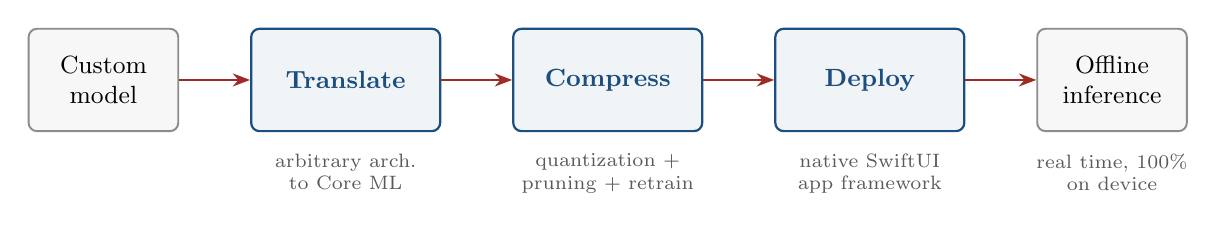
\begin{tikzpicture}[
  node distance=8mm and 9mm,
  stage/.style={draw=pipeblue, line width=0.8pt, rounded corners=3pt,
    fill=pipeblue!6, minimum width=24mm, minimum height=13mm,
    align=center, font=\small\bfseries, text=pipeblue},
  sub/.style={font=\scriptsize, text=black!65, align=center},
  io/.style={draw=black!45, line width=0.7pt, rounded corners=3pt,
    fill=black!3, minimum width=19mm, minimum height=13mm, align=center, font=\small},
  arr/.style={-{Stealth[length=2.2mm]}, line width=0.9pt, pipeaccent}]
\node[io] (model) {Custom\\model};
\node[stage, right=of model] (trans) {Translate};
\node[stage, right=of trans] (comp) {Compress};
\node[stage, right=of comp] (dep) {Deploy};
\node[io, right=of dep] (run) {Offline\\inference};
\draw[arr] (model) -- (trans);
\draw[arr] (trans) -- (comp);
\draw[arr] (comp) -- (dep);
\draw[arr] (dep) -- (run);
\node[sub, below=1.5mm of trans] {arbitrary arch.\\to Core ML};
\node[sub, below=1.5mm of comp] {quantization +\\pruning + retrain};
\node[sub, below=1.5mm of dep] {native SwiftUI\\app framework};
\node[sub, below=1.5mm of run] {real time, 100\%\\on device};
\end{tikzpicture}
\caption{The proposed pipeline. A custom vision model is translated to Core ML, automatically compressed, and deployed into a reusable native iOS application for real time, fully offline inference. Each stage is a scriptable, reusable step rather than a manual port.}
\label{fig:pipeline}
\end{figure*}

\section{Methods}
\subsection{Pipeline Overview}
The framework is organized as the four stage pipeline shown in Fig.~\ref{fig:pipeline}. A trained model enters the \emph{translate} stage, which converts it to the Core ML format. The \emph{compress} stage applies mixed precision quantization, structured pruning, and a short retraining pass to recover any lost accuracy. The \emph{deploy} stage embeds the resulting model in a native iOS application, and the \emph{run} stage performs inference entirely on the device. Because the application loads models through a generic interface, swapping in a new architecture does not require changes to the surrounding app code.

\subsection{Native iOS Application}
The application is built in Swift and SwiftUI using an MVVM architecture, with inference isolated behind a model independent module that bridges the camera feed to Core ML through Apple's Vision framework. We configured the Xcode build and signing toolchain to deploy to a physical iPhone, which is required to measure realistic on device throughput and latency. The YOLO family~\cite{redmon2016yolo} is used as the reference detector because of its strong accuracy to latency trade off; the current build uses a custom \texttt{yolo26n} model exported from the Ultralytics framework~\cite{ultralytics2023}.

\subsection{Model Compression and Evaluation}
To establish the compression stage, we built an automated quantize and evaluate script that converts a model from 16 bit floating point (FP16) to 8 bit integer (INT8) precision~\cite{jacob2018quant} and benchmarks the result. We evaluate three quantities against the uncompressed baseline: detection accuracy (precision and recall), on disk model size, and per image inference time, measured on a fixed set of 128 COCO validation images~\cite{lin2014coco}. This harness is model independent, so it will apply unchanged to future custom models.

\subsection{Target Application}
Our target application is on device detection of CD4+ T~cells for point of care immune monitoring. Dixit \emph{et al.}~\cite{dixit2025} demonstrate an AI enabled microfluidic cytometer in which a YOLO detector counts CD4+ T~cells labeled with antibody beads in microscope video of whole blood, with accuracy comparable to flow cytometry. In that work inference runs on a cloud GPU; porting the detector through our pipeline onto an iPhone would remove the cloud dependency and enable the portable, low resource operation the authors envision.

\section{Results (Partial)}
\subsection{On Device Deployment}
The custom \texttt{yolo26n} model was successfully deployed to a physical iPhone within our SwiftUI application and performs live object detection in real time, sustaining 30.3~frames per second at 13.1~ms per frame (Fig.~\ref{fig:detection}). Because the model was swapped in without modifying the application, this result validates the model independent loader and confirms that the hardest integration steps, physical device deployment and custom model loading, function end to end.

\subsection{Automated Quantization}
Table~\ref{tab:quant} and Fig.~\ref{fig:quant} report the measured effect of INT8 quantization. Model size fell by 74\% (9.9 to 2.6~MB) and per image inference time fell by 3.2$\times$ (16.5 to 5.2~ms), while precision and recall were essentially unchanged (precision 0.752 to 0.743; recall 0.534 to 0.540). Compression therefore yields a large efficiency gain at negligible accuracy cost on this workload.

\begin{table}[t]
\caption{Effect of INT8 Quantization (128 COCO images)}
\label{tab:quant}
\centering
\begin{tabular}{lccc}
\toprule
Metric & FP16 & INT8 & Change \\
\midrule
Precision        & 0.752 & 0.743 & 1.2\% lower \\
Recall           & 0.534 & 0.540 & 1.1\% higher \\
Model size (MB)  & 9.9   & 2.6   & 74\% smaller \\
Inference (ms)   & 16.5  & 5.2   & $3.2\times$ faster \\
\bottomrule
\end{tabular}
\end{table}

\begin{figure}[t]
\centering
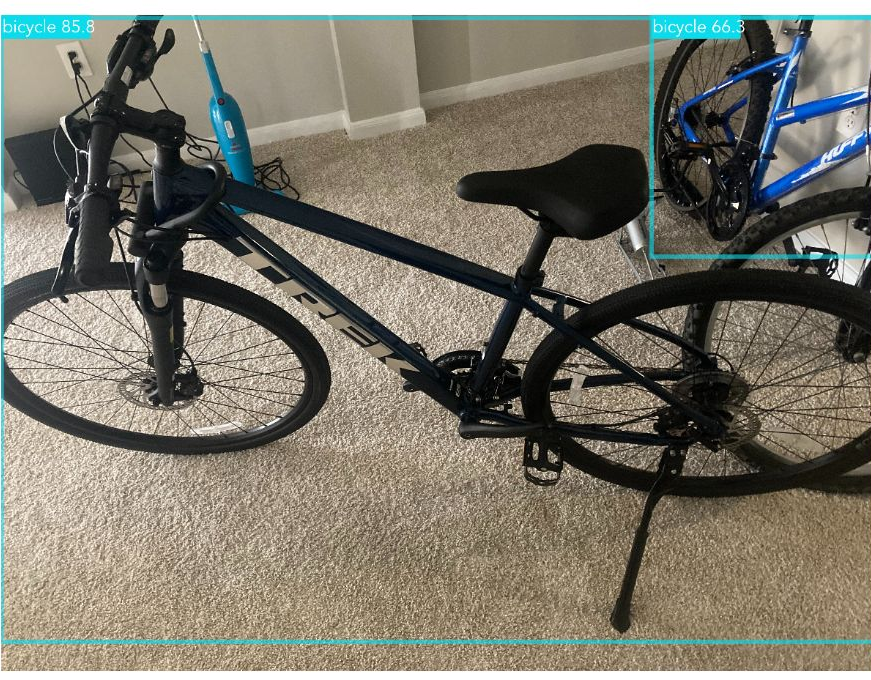
\includegraphics[width=\columnwidth]{figures/detection.png}
\caption{Custom \texttt{yolo26n} detector running fully on device in our iOS application, with per object confidence scores. The live camera build sustains 30.3~FPS (13.1~ms per frame).}
\label{fig:detection}
\end{figure}

\begin{figure*}[t]
\centering
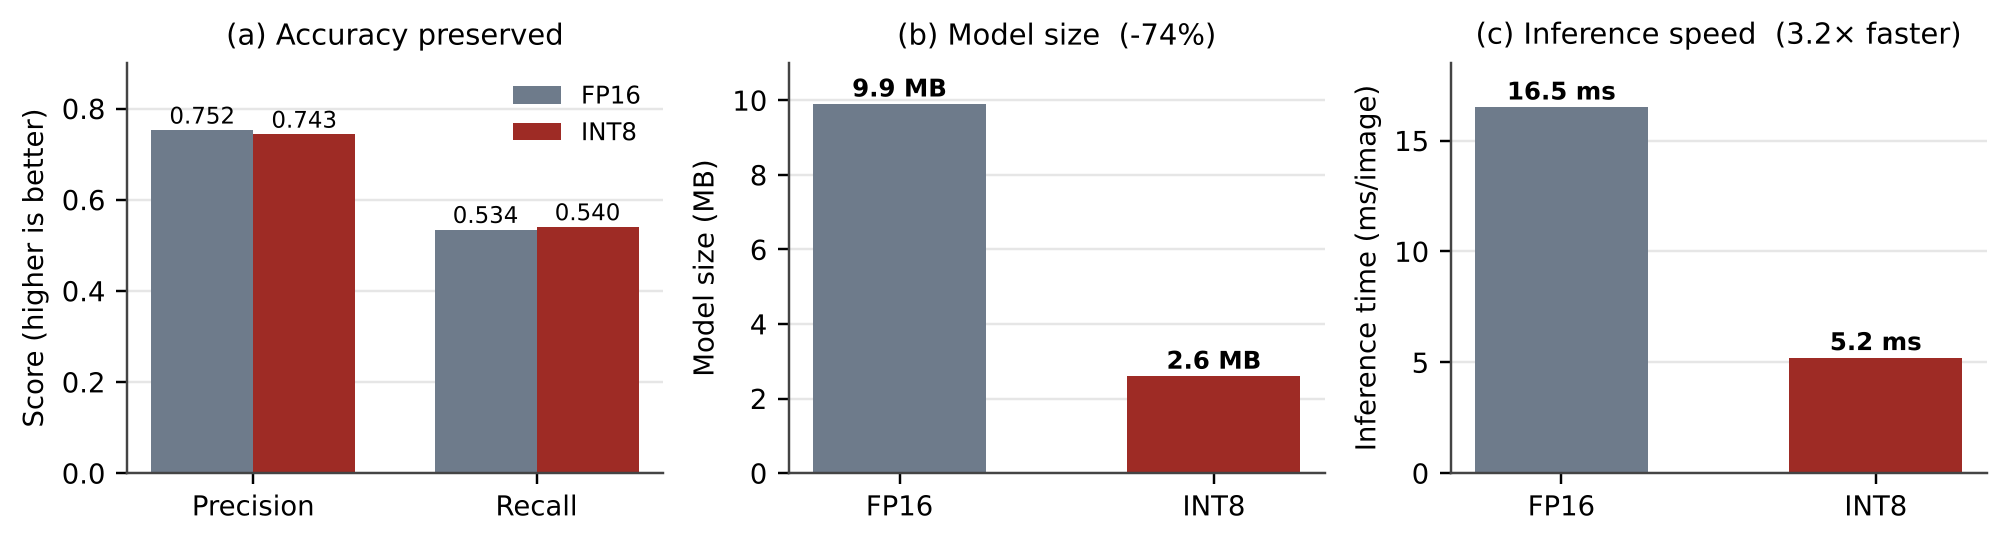
\includegraphics[width=\textwidth]{figures/quantization.png}
\caption{Measured impact of FP16 to INT8 quantization on a reference detector, evaluated on 128 COCO images: (a) precision and recall are preserved, (b) model size drops 74\%, and (c) inference is 3.2$\times$ faster. The same automated harness will be applied to future custom models.}
\label{fig:quant}
\end{figure*}

\section{Discussion (Partial)}
The partial results reduce the risk in the two most uncertain parts of the project. On device deployment of a custom model is working, and the compression stage already delivers substantial, automated efficiency gains with negligible accuracy loss, which is evidence that the project's end of semester targets (a 10$\times$ size reduction, $\leq$18~ms per frame inference, and $\geq$98.5\% of baseline accuracy) are realistic. Several limitations remain. The quantization results were obtained on a general detector and the standard COCO set, not yet on the target cell detection task; structured pruning and retraining are specified but not yet integrated into the automated stage; and the four stages are presently run in sequence rather than as a single scripted flow.

The next phase addresses these gaps in order: integrate pruning and retraining into the compression stage; train and convert a CD4+ T cell detector following the dataset and evaluation protocol of Dixit \emph{et al.}~\cite{dixit2025}, targeting mean average precision and cell count agreement comparable to the published cloud model; and deploy that detector on the iPhone, benchmarking on device latency and accuracy against the cloud baseline. Success would demonstrate a complete path from an arbitrary custom model to a private, offline, point of care diagnostic application.

\section*{Acknowledgements}
The author thanks Dr.~Vivek Boominathan for his guidance throughout this project, as well as the instructor and teaching staff of ELEC~594 at Rice University. This work makes use of the open source Ultralytics and Core ML tooling.

\section*{CRediT Author Statement}
\textbf{Anh Pham:} Conceptualization, Methodology, Software, Validation, Formal analysis, Investigation, Data curation, Visualization, Writing, original draft; Writing, review and editing. As a single author (team of one) project, all contributor roles were carried out by the author.

\bibliographystyle{IEEEtran}
\bibliography{refs}

\end{document}
